% This file was created with tikzplotlib v0.10.1.
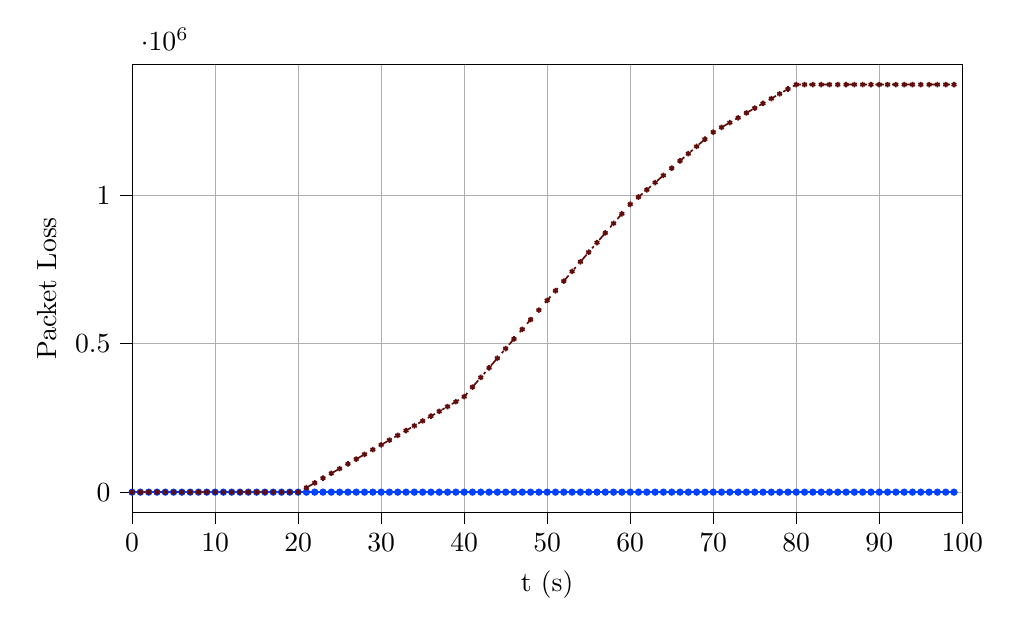
\begin{tikzpicture}

\definecolor{blue064255}{RGB}{0,64,255}
\definecolor{darkgrey176}{RGB}{176,176,176}
\definecolor{maroon971111}{RGB}{97,11,11}

\begin{axis}[
height=0.6\textwidth,
tick align=outside,
tick pos=left,
width=\textwidth,
x grid style={darkgrey176},
xlabel={t (s)},
xmajorgrids,
xmin=0, xmax=100,
xtick style={color=black},
y grid style={darkgrey176},
ylabel={Packet Loss},
ymajorgrids,
ymin=-68652.2, ymax=1441696.2,
ytick style={color=black}
]
\addplot [semithick, blue064255, mark=*, mark size=1, mark options={solid}]
table {%
0 0
1 0
2 0
3 0
4 0
5 0
6 0
7 0
8 0
9 0
10 0
11 0
12 0
13 0
14 0
15 0
16 0
17 0
18 0
19 0
20 0
21 0
22 0
23 0
24 0
25 0
26 0
27 0
28 0
29 0
30 0
31 0
32 0
33 0
34 0
35 0
36 0
37 0
38 0
39 0
40 0
41 0
42 0
43 0
44 0
45 0
46 0
47 0
48 0
49 0
50 0
51 0
52 0
53 0
54 0
55 0
56 0
57 0
58 0
59 0
60 0
61 0
62 0
63 0
64 0
65 0
66 0
67 0
68 0
69 0
70 0
71 0
72 0
73 0
74 0
75 0
76 0
77 0
78 0
79 0
80 0
81 0
82 0
83 0
84 0
85 0
86 0
87 0
88 0
89 0
90 0
91 0
92 0
93 0
94 0
95 0
96 0
97 0
98 0
99 0
};
\addplot [semithick, maroon971111, dash pattern=on 1pt off 3pt on 3pt off 3pt, mark=asterisk, mark size=1, mark options={solid}]
table {%
0 0
1 0
2 0
3 0
4 0
5 0
6 0
7 0
8 0
9 0
10 0
11 0
12 0
13 0
14 0
15 0
16 0
17 0
18 0
19 0
20 0
21 15137
22 31016
23 47111
24 63173
25 79182
26 95159
27 111177
28 127332
29 143342
30 159332
31 175350
32 191424
33 207498
34 223744
35 239981
36 256053
37 272294
38 288456
39 304614
40 321503
41 353955
42 386445
43 418780
44 451303
45 483731
46 516225
47 548690
48 581026
49 613490
50 645964
51 678445
52 710954
53 743437
54 775956
55 808313
56 840751
57 873269
58 905591
59 937842
60 969918
61 994275
62 1018586
63 1042858
64 1067219
65 1091574
66 1115942
67 1140269
68 1164638
69 1188976
70 1212696
71 1228881
72 1244913
73 1261144
74 1277373
75 1293595
76 1309729
77 1325940
78 1342022
79 1358107
80 1373044
81 1373044
82 1373044
83 1373044
84 1373044
85 1373044
86 1373044
87 1373044
88 1373044
89 1373044
90 1373044
91 1373044
92 1373044
93 1373044
94 1373044
95 1373044
96 1373044
97 1373044
98 1373044
99 1373044
};
\end{axis}

\end{tikzpicture}
